\chapter{Behavioural graph models}\label{sec:users-behaviors}

If we want to infer some information about a huge graph, such as the ones behind the web or social networks such as Facebook, we usually can't perform our computation directly on the real graph: it usually need an unsurmountable amount of time. Therefore, graph models are devised in order to represent them closely enough, and perform efficient analysis on them.

Some properties we usually are interested in when dealing with a network (or a graph) are:
\begin{itemize}
    \item the overall number of nodes,
    \item the average degree,
    \item the number of nodes with a certain degree,
    \item the size of the communities,
    \item the degree distribution.
\end{itemize}

\section{Erd\H{o}s–Rényi model}\label{sec:gnp}
    
This is a model for generating random graphs, that has many applications due to its simplicity, but doesn't fit real world networks: the nodes in such a generated graph have more or less the same degree, based on a fixed probability; in real networks degrees usually follow a gaussian distribution.

Denote by $\ergen(n, p)$ a random process that produces a graph with $n$ nodes, in which each edge appears with probability $p$. This process can be described by the following algorithm:
\begin{lstlisting}[caption = {The $\ergen(n,p)$ algorithm},
                    label   = {lst:gnp}]
Sample $\ergen(n,p)$:
    let $E := [n]$
    $E \gets \emptyset$
    for each $\{i, j\} \in \binom{V}{2}$:
        flip a coin with head probability $p$
        if the coin comes up head:
            $E \gets E \cup \{\{i,j\}\}$
    return $G(V,E)$
\end{lstlisting}

We are interested in studying how the graphs generated by this process change when $p$ changes.
    

\subsubsection{Degree distribution}\label{sec:gnp-degree}

We begin our study of a given graph $G$ obtained by $\ergen(n, p)$ looking at its degree distribution. Let $X = \deg(i) = \sum_{j \neq i} x_j$, where the $x_j$ are mutually independent RVs, and defined as:
\[
    x_j =
    \begin{cases}
        1 & \text{if } \exists i : \{i, j\} \in E(G) \text{\qquad (with probability } p)     \\
        0 & \text{otherwise}                         \text{\qquad \qquad \qquad (with probability } 1 - p) \\
    \end{cases}
\]
Note that from the perspective of any given vertex $v$, there are $\abs{V} - 1$ possible edges coming out of it, and are all governed by the same distribution; therefore:
\[
    \expval(\deg(v)) = \sum_{x \neq v} \Pr{\{v, x\} \in E(G)} = \sum_{x \neq v} p = (n - 1) p
\]
\todo{

It can be valuable to get a better visual in how the degree distributes, or better, to discover that it is actually \emph{concentrated} around the average. Thanks to the mutual independence of the $x_j$, we can apply the Chernoff Bound [\ref{chernoff2}] to prove such claim:
\[
    X = \sum x_j = \frac{n}{2} \pm \sqrt{n \ln \frac{1}{\delta}} \text{ with probability } 1 - O(\delta)
\]

Thus, since in average each node has the same degree, $G(n,p)$ produces \textit{almost regular graphs}, that are not suitable for representing real world social graphs, as stated at the beginning of this section.
}


\subsubsection{Connectivity}

Up next is the analysis for which probability $p$ the generator $\ergen(n, p)$ will produce a connected graph. Before starting, we introduce a combinatorial property that will be useful later:

\begin{lem}\label{l:gnp-connectivity}
    If for every nontrivial subset of \,$V$ there is an edge of \,$G$ ``crossing'' it, then the graph is connected:
    \[
        \forall\; \emptyset \subset S \subset V \; \exists \{u,v\} \in E : u \in S \wedge v \in V \setminus S \implies G \text{ is connected}  
    \]
\end{lem}

\begin{figure}[ht]
    \centering
    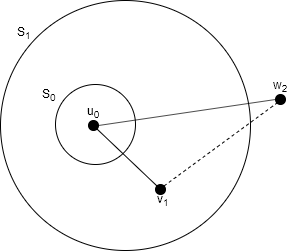
\includegraphics[scale=0.5]{gnp_l1}
    \caption{Proof visualization of lemma \ref{l:gnp-connectivity}}
    \label{fig:gnp-l1}
\end{figure}

\todo{

\begin{proof}[Proof (Idea)] This is proven by induction on the subsets of a given graph G, and is visualized in figure [\ref{fig:gnp-l1}]:
    \begin{itemize}
        \item Base step: In $S_0$ there is only the node $u_0$, so there must be an edge from $u_0$ to a node $v_1 \in V-S$;
        \item Inductive step: Go on expanding the frontier (the set of nodes in $S$ that have an edge connecting them to a node in $V \setminus S$) until the BFS visit reaches all the nodes. \qedhere
    \end{itemize}
\end{proof}
}

With this lemma, a claim on connectivity can be made:

\begin{thm}[Connectivity of $G(n,p)$]\label{thm:gnp-connectivity}
    Let $G$  be a graph generated by $\ergen(n, p)$. If $p \geq \frac{8 \ln n}{n}$, then $G$ is connected with probability at least $1 - \frac{1}{n}$.
\end{thm}

\begin{proof}
    Let $\xi_S$ be the event ``there are no edges crossing the bipartition $(S, V \setminus S)$ of the graph $G$'' for each proper nonempty subset $S$ of $V$. By the previous lemma, we can deduce that that:
    \[
        \Pr{G \text{ is not connected}} = \Pr{\bigvee_{S \subset V} \xi_S}
    \]
    
    Note that there are $2^n - 2$ of such subsets, but we are interested only in half of the corresponding events, since each event $\xi_S$ will have its own corresponding event $\xi_{V \setminus S}$, and both of them essentially represent the same event: in other words,  $\xi_S$ and $\xi_{V \setminus S}$ are not independent. To correct this caveat it is sufficient to only consider one fixed half of the events, and here they are conveniently chosen such that $|S| \leq \frac{|V|}{2}$.
    
    Let $n = |V|$ and $s = |S|$. Observe that there are $|S| \cdot |V \setminus S|$ possible edges from $S$ to $V \setminus S$, each of which will not be in the graph with probability $1 - p$; also, since $S$ is a subset of $V$, then $|S| \cdot |V \setminus S| = s \cdot (n - s)$. Putting the pieces together, the probability of a single event $\xi_S$ is obtained as:
    \begin{align*}
        \Pr{\xi_S} &= (1 - p)^{s \cdot (n - s)}                   &                                  \\
        &\leq e^{-p \cdot s \cdot (n - s)}                        & \tag{by inequality \ref{eq:e-x}} \\
        &\leq e^{-p \cdot s \cdot n/2}                            & \tag{since $s \leq \frac{n}{2}$} \\
        &\leq e^{-\frac{8 \ln n}{n} \cdot s \cdot \frac{n}{2}}    &                                  \\
        &= \left(e^{-\ln n} \right)^{4 \cdot s} = n^{-4 \cdot s}  & 
    \end{align*}
    
    Now, let's fix $s$ to a specific value, and consider the probability that $\xi_S$ happens for any $S \subset V$ with cardinality $s$:
    \begin{align*}
        \Pr{\exists S \in \binom{V}{s} : \xi_S} &\leq \sum_{S \in \binom{V}{s}} \Pr{\xi_S} & \tag{by the union bound \ref{eq:union-bound}}               \\
        &\leq \sum_{S \in \binom{V}{s}} n^{-4s} = \binom{n}{s} \cdot n^{-4s}               & \tag{since $\displaystyle \abs{\binom{V}{s}} = \binom{n}{s}$} \\
        &\leq n^s \cdot n^{-4s} = n^{-3s}                                                  & \tag{since $\displaystyle \binom{n}{s} \leq n^s$}
    \end{align*}
    
    Now we are ready to compute the probability that a graph $G$ obtained using $\ergen(n, p)$ is connected. To do that we will distribute the subsets $S$ in \emph{buckets}, according to their cardinality:
    \begin{align*}
        \Pr{G \text{ is not connected}} &= \Pr{\bigcup_{S \subset V} \xi_S}         & \\
        &= \Pr{\exists s \in \{1, \ldots, n\} : \exists S \in \binom{V}{s} : \xi_S} & \\
        &\leq \sum_{s = 1}^{n/2} n^{-3s}                                            & \tag{by the union bound \ref{eq:union-bound}}\\
        &\leq \sum_{s = 1}^{n/2} n^{-3} = \frac{1}{2n^2}                            &
    \end{align*}
    
   By complementing the result, it entails that $\Pr{G \text{ is connected}} \geq 1 - \frac{1}{2n^2} \geq 1 - \frac{1}{n}$, which is even a stronger claim than the one stated by the theorem.
\end{proof}

The theorem we just proved is also known as a \emph{zero-one law}: it holds for the given bound of $p$, but it ceases to hold almost immediately when $p$ crosses it, so $p = \frac{8 \ln n}{n}$ is sort of a threshold between generators $\ergen(n, p)$ that produce connected graphs with high probability and generators that produce disconnected graphs with high probability.

We won't prove exactly what we just claimed, since it would be hard, but something weaker:
\begin{thm}
    If $p < \frac{\varepsilon}{n} \ll \frac{8 \ln n}{n}$, then $G(n, p)$ is disconnected with probability $\geq 1 - \varepsilon$.
\end{thm}

\begin{proof}
    Let $X := \deg(i)$ and $x_j$ defined as before (see [\ref{sec:gnp-degree}]).
    \begin{enumerate}
        \item $X = \sum_{j \neq i} x_j = \sum_{j \neq i} \Pr{\{ i,j \} \in E(G)}$;
        \item We know by hypothesis that $\mathbb{E}[X_j] = p < \frac{\varepsilon}{n}$;
        \item $\mathbb{E}[X] < (n-1) \frac{\varepsilon}{n}$;
        \item $\Pr{X \geq \frac{1}{\varepsilon} \cdot \mathbb{E}[X]} \leq \varepsilon$ (by Markov inequality [\ref{eq:markov2}]);
        \item Since $\frac{1}{\varepsilon} \cdot \mathbb{E}[X] \approx 1$ and $X$ has integer values, we can write the previous expression as \\
        $\Pr{X > 0} \leq \varepsilon$, and this is the probability that exists a node $i$ that has at least one neighbor;
        \item Thus, by complement, $\Pr{\exists\ i \st i \in V \text{ and } i \text{ has 0 neighbors}} = \Pr{G(n,p) \text{ is not connected}} \geq 1 - \varepsilon$.
    \end{enumerate}
\end{proof}
    

\subsection{Diameter}

It is known that graphs generated by $\ergen(n,p)$ have small diameter with high probability. The proof is left as an exercise.


\section[Preferential attachment]{Preferential attachment\raisebox{.3\baselineskip}{\normalsize\footnotemark}}
\footnotetext{Part of this section is taken from \href{https://github.com/Halolegend94/uni_social_behavioral_networks/blob/master/chapters/ch04-random-graphs.tex}{this repo} by \href{https://github.com/Halolegend94}{Cristian Di Pietrantonio}.}\label{sec:pref-att}
    
\textit{Preferential attachment} is another model for generating random graphs, but it follows the rule ``the rich get richer'', meaning that nodes with higher degree will see their degree becoming higher and higher.

The preferential attachment is a generative (or sequential) model, and the rule used to build a graph is the following: you begin with a single node with a self loop, when you have built a graph with $N-1$ nodes, you add the $N$-th node with an edge that goes from $N$ to a node $i$ chosen accordingly with a probability proportional to the degree of $i$.

There exist many variants of this model, for example with each node creating $k$ edges instead of one, with no self-loops, etc.

\begin{figure}
    \centering
    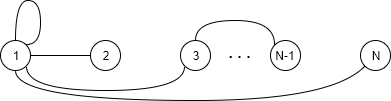
\includegraphics[scale=0.7]{preferential-attach}
    \caption{Example of a graph generated by the preferential attachment model}
    \label{fig:pref-att}
\end{figure}

The graphs generated by the Preferential attachment model follow a power law degree distribution, like the one observed in many real world networks, indeed, the fraction of nodes of degree $x$ approaches $x^{-3}$.\\
This characteristic causes that this model fits well with social and biological networks, so it can be used to develop efficient algorithms that actually work in practice.

Now we give a general definition of power law:
\begin{defn}[Power law]
    A power law is a functional relationship $y = ax^{-c}$ between two quantities, where one quantity varies as a power of the other.
\end{defn}

As a consequence of the definition, we get that a power law appears as a line in a log log scale plot, as can be seen in fig. \ref{fig:power-law}.

\begin{figure}
    \centering
    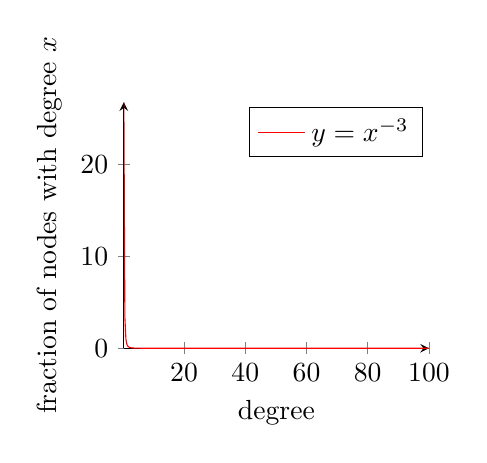
\begin{tikzpicture}
        \begin{axis}[
            width=0.45\textwidth,
            axis lines = left,
            xlabel = degree,
            ylabel = {fraction of nodes with degree $x$},
        ]
        \addplot [
            domain=0:100, 
            samples=300, 
            color=red,
        ]{1/(x^3)};
        \addlegendentry{$y=x^{-3}$}
        \end{axis}
    \end{tikzpicture}
    \hskip 7pt
    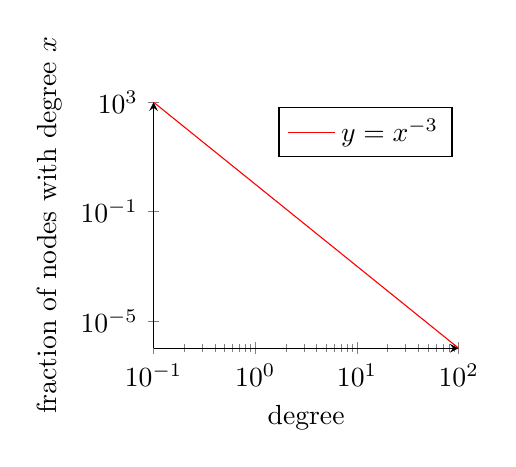
\begin{tikzpicture}
        \begin{axis}[
            width=0.45\textwidth,
            xmode=log,
            ymode=log,
            axis lines = left,
            xlabel = degree,
            ylabel = {fraction of nodes with degree $x$},
        ]
        \addplot [
            domain=0.1:100,
            samples=300,
            color=red,
        ]{1/(x^3)};
        \addlegendentry{$y=x^{-3}$}
        \end{axis}
    \end{tikzpicture}
    \caption{Power law distribution with linear and log log scale}
    \label{fig:power-law}
\end{figure}

In the social network context it means that it is exponentially more likely to pick ``normal people'' with few friends or followers rather than popular profiles, called ``celebrities'' or ``authorities''.\\
Nodes with high degree in a social network are few, but they exists. So, as an example, an advertisement agency could pay those celebrities to publicize a product, enabling a spread of information due to the high number of connections those nodes have.
    
    
\subsection{Formalization}\label{sec:pref-attach-formalization}

    Inductive definition of the model:
    \begin{itemize}
        \item Base step: $G_1$ is a single node with a self loop;
        \item Inductive step (for $i = 2, 3, \ldots$):
        \begin{enumerate}
            \item add node $i$ to $G_i$;
            \item add a ``\textit{half edge}'' coming out from node $i$;
            \item choose a node $j$ randomly, with probability proportional to its degree:
            \[
                \Pr{\text{neighbor of $N$ is $i$}} = \frac{deg(i)}{\sum_{k=1}^{N} deg(k)}
            \], where the denominator is a normalization factor;
            \item close the \textit{half edge} from $i$, by connecting it to $j$.
        \end{enumerate}
    \end{itemize}
    
    Note that there are many possible configurations from the second step onwards, and the probability of each of them depends on the degrees of the nodes (where a loop counts twice and a self loop once). We can see the possible configurations with their respective probabilities in picture [\ref{fig:pref-att-steps}].
    
    \begin{figure}[h!]
        \centering
        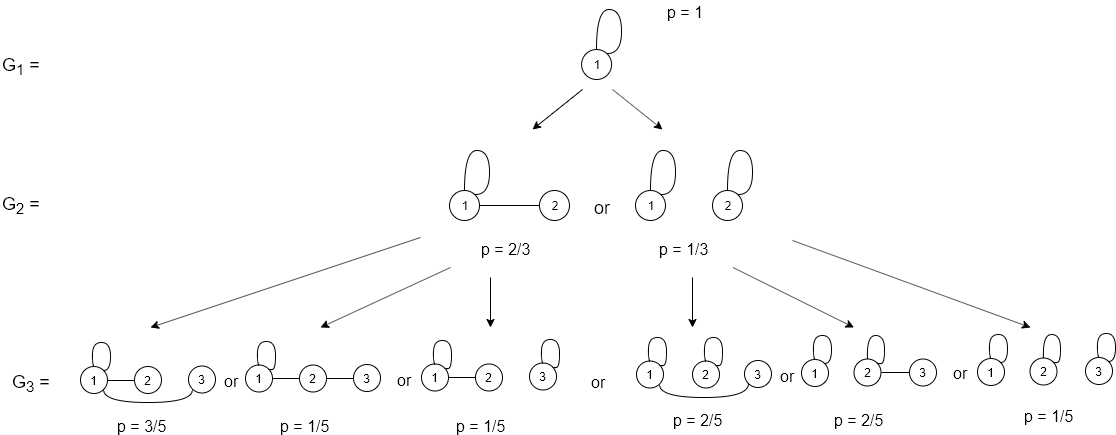
\includegraphics[width=\textwidth]{pref-attach-steps}
        \caption{Example of a graph generated by the preferential attachment model}
        \label{fig:pref-att-steps}
    \end{figure}


\subsection{Degree distribution}\label{sec:pref-attach-degree}

    We are interest in studying the degree distribution of the graphs generated by the preferential attachment model, so that we can show that it follows a power low, as previously claimed.
    
    We begin with what we already know from the definition of the model.
    
    \obs $\abs{V(G_t)} = t$.
    
    \obs $\abs{E(G_t)} = t$.
    
    \obs There are no node of degree zero.
    
    \obs $\Pr{v_{t+1} \sim v_i} = \Pr{\{ v_{t+1}, v_i \} \in E(G_{t+1})} = \frac{\deg_{G_t}(v_i)}{2t+1}$.
    
    \obs $\Pr{v_{t+1} \sim v_{t+1}} = \frac{1}{2t+1}$.
    
    Now, our claim about the degree distribution.
    
    \begin{thm}\label{thm:pref-attach-degree}
        Let $X_t^{\left(d\right)}$ be the number of nodes that have degree $d$ in $G_t$, then \\ $E\left[X_t^{\left(d\right)}\right] = t \cdot \frac{4}{(d+2) \cdot (d+1) \cdot d} \pm O(1)$.
    \end{thm}

    Note that is meaningful to study the expected value because the random variable $X$ is concentrated.
    
    \obs $\lim_{d \to \infty}$ $\frac{\frac{4}{(d+2) \cdot (d+1) \cdot d}}{d^{-3}} = \Theta(1)$, in other words $E\left[X_t^{\left(d\right)}\right]^{d \to \infty} \to t \cdot d^{-3}$.
    
    We are going to demonstrate the theorem by double induction, on the degree $d$ and on the time $t$, so we fix the degree and we study the number of nodes when $t$ changes.
    
    For this proof, we have two base steps and an inductive step, for each of which we have different possible possibilities for the new node $v_{t+1}$:
    \begin{enumerate}
        \item Base step 1 ($d = 1$):
            \begin{enumerate}
                \item $v_{t+1}$ creates a self loop, so the number of nodes with $\deg=1$ doesn't change,
                \item $v_{t+1}$ connects itself with a node of degree 1, in this case $v_{t+1}$ is a new node with $\deg=1$, but the other node now have a greater degree, so the overall number of nodes with $\deg=1$ does not change,
                \item $v_{t+1}$ connects itself with a node of degree 2 or more, in this case $v_{t+1}$ is a new node with $\deg=1$, so the number of nodes with $\deg=1$ increases by one;
            \end{enumerate}
        \item Base step 2 ($d = 2$):
            \begin{enumerate}
                \item $v_{t+1}$ creates a self loop, so the number of nodes with $\deg=2$ increases by one,
                \item $v_{t+1}$ connects itself with a node of degree 1, so the number of nodes with $\deg=2$ increases by one,
                \item $v_{t+1}$ connects itself with a node of degree 2, so the number of nodes with $\deg=2$ decreases by 1 (since now that node has a greater degree),
                \item $v_{t+1}$ connects itself with a node of degree 3 or more, so the number of nodes with $\deg=2$ does not change;
            \end{enumerate}
        \item Inductive step ($d \geq 3$):
            \begin{enumerate}
                \item $v_{t+1}$ connects itself with a node of degree $d-1$, so the number of nodes with $\deg=d$ increases by one,
                \item $v_{t+1}$ connects itself with a node of degree $d$, so the number of nodes with $\deg=d$ decreases by one (since now that node has a greater degree),
                \item $v_{t+1}$ connects itself to any other node, so the number of nodes with $\deg=d$ does not change.
            \end{enumerate}
    \end{enumerate}
    
\subsubsection{\large{Base step 1: $d = 1$.}}
    
    Since $G_{t+1}$ depends on $G_t$, $\forall\ t = 1,2,\ldots$, we will need to condition on all the previous random choices.
    
    \begin{lem}\label{l:pref-att-1}
        \begin{flalign}
            &E\left[ X_{t+1}^{\left(1\right)} \st X_{t}^{\left(1\right)} = x \right] = (x+1) \cdot \left( 1 - \frac{1}{2t+1} \right)&
        \end{flalign}
    \end{lem}
    \begin{proof}
        \begin{flalign*}
            E\left[ X_{t+1}^{\left(1\right)} \st X_{t}^{\left(1\right)} = x \right] &=
            \Pr{X_{t+1}^{\left(1\right)} = x} \cdot x + \Pr{X_{t+1}^{\left(1\right)} = x+1} \cdot (x+1)&\\
            &= \frac{x + 1}{2t + 1} \cdot x + \frac{(2t+1) - (x+1)}{2t+1} \cdot (x+1)&\\
            &= \frac{x+1}{2t+1} \cdot \left( x - (x+1) \right) + \frac{2t+1}{2t+1} (x+1)&\\
            &= - \frac{x+1}{2t+1} + (x+1)&\\
            &= (x+1) \cdot \left( 1 - \frac{1}{2t+1} \right)&
        \end{flalign*}
    \end{proof}

    \begin{lem}\label{l:pref-att-2}
        \begin{flalign}
            &E\left[ X_{t+1}^{\left(1\right)} \right] = \left( E\left[ X_{t}^{\left(1\right)} \right] +1 \right) \cdot \left( 1 - \frac{1}{2t+1} \right)&
        \end{flalign}
    \end{lem}
    \begin{proof}
        \begin{flalign*}
            E\left[ X_{t+1}^{\left(1\right)} \right] &=
            \sum_{x \geq 0} \left( \Pr{X_{t}^{\left(1\right)} = x} \cdot E\left[ X_{t+1}^{\left(1\right)} \st X_{t}^{\left(1\right)} = x \right] \right)&\\
            &= \sum_{x \geq 0} \left( \Pr{X_{t}^{\left(1\right)} = x} \cdot (x+1) \cdot \left( 1 - \frac{1}{2t+1} \right) \right)&
            \tag{by \href{https://en.wikipedia.org/wiki/Law_of_total_expectation}{\textit{law of total expectation}} and lemma [\ref{l:pref-att-1}]}\\
            &= \left( 1 - \frac{1}{2t+1} \right) \cdot \sum_{x \geq 0} \left( \Pr{X_{t}^{\left(1\right)} = x} \cdot (x+1) \right)&\\
            &= \left( 1 - \frac{1}{2t+1} \right) \cdot \left( \mathunderline{red}{\sum_{x \geq 0} \left( \Pr{X_{t}^{\left(1\right)} = x} \cdot x \right)} + \mathunderline{green}{\sum_{x \geq 0} \left( \Pr{X_{t}^{\left(1\right)} = x} \right)} \right)&\tag{by distributive law}\\
            &= \left( 1 - \frac{1}{2t+1} \right) \cdot \left( \mathunderline{red}{E\left[ X_{t}^{\left(1\right)} \right]} + \mathunderline{green}{1} \right)&
            \tag{since the green part corresponds to the probability that $X_t^{\left(1\right)}$ assumes any non negative value, that is 1}
        \end{flalign*}
    \end{proof}
    
    \begin{lem}\label{l:pref-att-3}
        \begin{flalign}
            &\exists\ c > 0 \text{ s. t. } \forall\ t\geq 0,\ \frac{2}{3} (t+1) -c \leq E\left[ X_{t+1}^{\left(1\right)} \right] \leq \frac{2}{3} (t+1) +c&
        \end{flalign}
    \end{lem}
    \begin{proof}[Proof by induction] \
        
        \textbf{Base step}, with $t=0$:\\
        At time $t+1$ the graph is $G_1$ and is composed by a single node with degree 2, as previously described (see [\ref{fig:pref-att-steps}]), so the claim holds for $c \geq \frac{2}{3}$:
        \begin{flalign*}
            &\frac{2}{3} -c \leq E\left[ X_{1}^{\left(1\right)} \right] = 0 \leq \frac{2}{3} +c&
        \end{flalign*}
        
        \textbf{Inductive step for the upper bound}: suppose that the claim holds for $E\left[ X_{t}^{\left(1\right)} \right]$,
        \begin{flalign*}
            E\left[ X_{t+1}^{\left(1\right)} \right] &= \left( E\left[ X_{t}^{\left(1\right)} \right] +1 \right) \cdot \left( 1 - \frac{1}{2t+1} \right)&\tag{by lemma [\ref{l:pref-att-2}]}\\
            &\leq \left( \frac{2}{3}t + c + 1 \right) \cdot \left( 1 - \frac{1}{2t+1} \right)&\tag{by inductive hypothesis}\\
            &= \left( 1 - \frac{1}{2t+1} \right) \cdot \left( \frac{2}{3}t + c \right) + \left( 1 - \frac{1}{2t+1} \right)&\\
            &\leq \left( 1 - \frac{1}{2t+1} \right) \cdot \left( \frac{2}{3}t + c \right) + 1&\tag{since $1 - \frac{1}{2t+1} \leq 1$}\\
            &= \frac{2}{3} t + c - \frac{2t}{3(2t+1)} - \frac{c}{2t+1} +1&\\
            &= \frac{2}{3} t + c - \frac{2t}{6t+3} - \frac{c}{2t+1} +1&\\
            &= \frac{2}{3} t + \left( 1 - \frac{2t}{6t+3} \right) + c \cdot \left( 1 - \frac{1}{2t+1} \right)&\\
            &= \frac{2}{3} t + \frac{4t + 3}{6t+3} + c \cdot \left( 1 - \frac{1}{2t+1} \right)&\\
            &= \frac{2}{3} t + \left(\frac{4t + 2}{6t+3} + \frac{1}{6t+3}\right) + c \cdot \left( 1 - \frac{1}{2t+1} \right)&\\
            &= \frac{2}{3} (t+1) + c - \frac{c}{2t+1} + \frac{1}{6t+3}&
            \tag{since $\frac{4t + 2}{6t+3} = \frac{2}{3}$}\\
            &\leq \frac{2}{3} (t+1) + c&\tag{since, for $c \geq \frac{1}{3},\ - \frac{c}{2t+1} + \frac{1}{6t+3} \leq 0$}
        \end{flalign*}
        
        \textbf{Inductive step for the lower bound}: suppose that the claim holds for $E\left[ X_{t}^{\left(1\right)} \right]$,
        \begin{flalign*}
            E\left[ X_{t+1}^{\left(1\right)} \right] &= \left( E\left[ X_{t}^{\left(1\right)} \right] +1 \right) \cdot \left( 1 - \frac{1}{2t+1} \right)&\tag{by lemma [\ref{l:pref-att-2}]}\\
            &\geq \left( \frac{2}{3}t - c + 1 \right) \cdot \left( 1 - \frac{1}{2t+1} \right)&\tag{by inductive hypothesis}\\
            &= \frac{2}{3}t + 1 - \frac{2t}{6t+3} - c \left( 1 - \frac{1}{2t+1} \right) - \frac{1}{2t+1}&\\
            &= \frac{2}{3}t + \left( 1 - \frac{2t}{6t+3} - \frac{1}{2t+1} \right) - c \left( 1 - \frac{1}{2t+1} \right)&\\
            &= \frac{2}{3}t + \left( \frac{6t + 3 - 2t -3}{6t+3} \right) - c \left( 1 - \frac{1}{2t+1} \right)&\\
            &= \frac{2}{3}t + \frac{4t}{6t+3} - c \left( 1 - \frac{1}{2t+1} \right)&\\
            &= \frac{2}{3}t + \underbrace{ \frac{4t}{6t+3} + \frac{2}{6t+3}}_{2/3} - \frac{2}{6t+3} - c - \frac{c}{2t+1}&\\
            &= \frac{2}{3} (t+1) -c + \frac{3c -2}{6t+3}&\\
            &\geq \frac{2}{3} (t+1) -c&\tag{since, for $c \geq \frac{2}{3},\ \frac{3c -2}{6t+3} \geq 0$}
        \end{flalign*}
    \end{proof}

\subsubsection{\large{Base step 2: $d = 2$.}}

    \begin{lem}\label{l:pref-att-4}
        \begin{flalign}
            &E\left[ X_{t+1}^{\left(2\right)} \st X_{t}^{\left(2\right)} = x,\ X_{t}^{\left(1\right)} = y \right] = x \cdot \left( 1 - \frac{2}{2t+1} \right) + y \cdot \frac{1}{2t + 1} + \frac{1}{2t + 1}&
        \end{flalign}
    \end{lem}
    \begin{proof}
        \begin{flalign*}
            &E\left[ X_{t+1}^{\left(2\right)} \st X_{t}^{\left(2\right)} = x,\ X_{t}^{\left(1\right)} = y \right] =&\\
            &= \mathunderline{red}{\Pr{\parbox{\textwidth/2}{node $t+1$ connects itself to some node that had degree 1 in $G_t$ or to $t+1$ itself} \st X_{t}^{\left(2\right)} = x,\ X_{t}^{\left(1\right)} = y}} \cdot (x+1) &\tag{we are adding a new node of degree 2}\\
            &\ \ \ + \mathunderline{green}{\Pr{\parbox{\textwidth/2}{node $t+1$ connects itself to some node that had degree 2 in $G_t$} \st X_{t}^{\left(2\right)} = x,\ X_{t}^{\left(1\right)} = y}} \cdot (x-1)&\tag{we are loosing a node of degree 2}\\
            &\ \ \ + \mathunderline{purple}{\Pr{\parbox{\textwidth/2}{node $t+1$ connects itself to some node that had degree $\geq 3$ in $G_t$} \st X_{t}^{\left(2\right)} = x,\ X_{t}^{\left(1\right)} = y}} \cdot x&\tag{the number of nodes of degree 2 does not change}\\
            &= \mathunderline{red}{\left( y \cdot \frac{1}{2t+1} + \frac{1}{2t+1} \right)} \cdot (x+1)
            + \mathunderline{green}{\left( x \cdot \frac{2}{2t+1} \right)} \cdot (x-1)
            + \mathunderline{purple}{\left( 1 - y \cdot \frac{1}{2t+1} - \frac{1}{2t+1} - \frac{2x}{2t+1} \right)} \cdot x&\tag{since we have three disjoint events, where the third one is the complement of the first two}\\
            &= \frac{y+1}{2t+1}x + \frac{y+1}{2t+1} + \frac{2x}{2t+1}x - \frac{2x}{2t+1} + \left( 1 - \frac{y+1}{2t+1} - \frac{2x}{2t+1} \right)&\\
            &= x - \frac{2x}{2t+1} + \frac{y+1}{2t+1}&\\
            &= x \cdot \left( 1 - \frac{2}{2t+1} \right) + \frac{y+1}{2t+1}&
        \end{flalign*}
    \end{proof}

    \begin{lem}\label{l:pref-att-5}
        \begin{flalign}
        &E\left[ X_{t+1}^{\left(2\right)} \right] = E\left[ X_{t}^{\left(2\right)} \right] \cdot \left( 1 - \frac{2}{2t+1} \right) + \frac{E\left[ X_{t}^{\left(1\right)} \right] +1}{2t + 1}&
        \end{flalign}
    \end{lem}
    \begin{proof}
        It is possible to prove this lemma explicitly with a procedure similar to the one used for lemma [\ref{l:pref-att-2}], but here we will present a more compact (implicit) proof:
        \begin{flalign*}
            &E_{X_t^{(2)}=x} \left[ E_{X_t^{(1)}=y \st X_t^{(2)}=x} \left[ x \cdot \left( 1 - \frac{2}{2t+1} \right) + \frac{y+1}{2t+1} \right] \right]&
        \end{flalign*}
        Note that this is possible because the expected value is linear and (in this case) also its value is linear with respect to $x$ and $y$.
    \end{proof}

    Now we are going to use the bounds found for $E\left[X_t^{(1)}\right]$ in lemma [\ref{l:pref-att-3}] to proof similar bounds for $E\left[X_{t+1}^{(2)}\right]$.
    
    \begin{lem}\label{l:pref-att-6}
        \begin{flalign}
        &\exists\ c > 0 \text{ s. t. } \forall\ t\geq 0,\ \frac{1}{6} (t+1) -c \leq E\left[ X_{t+1}^{\left(2\right)} \right] \leq \frac{1}{6} (t+1) +c&
        \end{flalign}
    \end{lem}
    \begin{proof}[Proof by induction] \
        
        \textbf{Base step}, with $t=0$:\\
        At time $t+1$ the graph is $G_1$ and is composed by a single node with degree 2, as previously described (see [\ref{fig:pref-att-steps}]), so the claim holds for $c \geq \frac{5}{6}$:
        \begin{flalign*}
        &\frac{1}{6} -c \leq E\left[ X_{1}^{\left(2\right)} \right] = 1 \leq \frac{1}{6} +c&
        \end{flalign*}
        
        \textbf{Inductive step for the upper bound}: suppose that the claim holds for $E\left[ X_{t}^{\left(2\right)} \right]$,
        \begin{flalign*}
        E\left[ X_{t+1}^{\left(2\right)} \right] &= E\left[ X_{t}^{\left(2\right)} \right] \cdot \left( 1 - \frac{2}{2t+1} \right) + \frac{E\left[ X_{t}^{\left(1\right)} \right]+1}{2t + 1}& \tag{by lemma [\ref{l:pref-att-5}]}\\
        &\leq \left( \frac{t}{6} + c \right) \cdot \left( 1 - \frac{2}{2t+1} \right) + \frac{\frac{2t}{3}+c+1}{2t + 1}&
        \tag{\parbox{\textwidth/3}{by inductive hypothesis and upper bound given by [\ref{l:pref-att-3}]}}\\
        &= \frac{t}{6} - \mathunderline{red}{\frac{1}{2t+1} \cdot \frac{t}{3}} + \mathunderline{green}{c \cdot \left( 1 - \frac{2}{2t+1} \right)} + \mathunderline{purple}{\frac{2t}{3} \cdot \frac{1}{2t+1}} + \mathunderline{green}{\frac{c}{2t+1}} + \frac{1}{2t+1}&\\
        &= \frac{t}{6} + \frac{1}{2t+1} \cdot \left( \mathunderline{purple}{\frac{2}{3}t} - \mathunderline{red}{\frac{1}{3}t} \right) + \mathunderline{green}{c \cdot \left( 1 - \frac{2-1}{2t+1} \right)} + \frac{1}{2t+1}&\\
        &= \frac{t}{6} + \mathunderline{cyan}{\frac{1}{2t+1} \cdot \frac{t}{3}} + c \cdot \left( 1 - \frac{1}{2t+1} \right) + \mathunderline{cyan}{\frac{1}{2t+1}}&\\
        &= \frac{t}{6} + \mathunderline{cyan}{\frac{t}{6t+3} + \frac{3}{6t+3}} + c \cdot \left( 1 - \frac{1}{2t+1} \right)&\\
        &= \frac{t}{6} + \mathunderline{cyan}{\frac{t+1/2}{6t+3} + \frac{5/2}{6t+3}} + c \cdot \left( 1 - \frac{1}{2t+1} \right)&\\
        &= \frac{t+1}{6} + \frac{5/2}{6t+3} + c - \frac{3c}{6t+3}& \tag{since $\frac{t+1/2}{6t+3} = \frac{1}{6}$}\\
        &\leq \frac{t+1}{6} + c& \tag{since $\frac{5/2}{6t+3} - \frac{3c}{6t+3} \leq 0$ if $c \geq \frac{5}{6}$}
        \end{flalign*}
        
        \textbf{Inductive step for the lower bound}: suppose that the claim holds for $E\left[ X_{t}^{\left(2\right)} \right]$,
        \begin{flalign*}
            E\left[ X_{t+1}^{\left(2\right)} \right] &= E\left[ X_{t}^{\left(2\right)} \right] \cdot \left( 1 - \frac{2}{2t+1} \right) + \frac{E\left[ X_{t}^{\left(1\right)} \right]+1}{2t + 1}& \tag{by lemma [\ref{l:pref-att-5}]}\\
            &\geq \left( \frac{t}{6} - c \right) \cdot \left( 1 - \frac{2}{2t+1} \right) + \frac{\frac{2t}{3}-c+1}{2t + 1}&
            \tag{\parbox{\textwidth/3}{by inductive hypothesis and lower bound given by [\ref{l:pref-att-3}]}}\\
            &= \frac{t}{6} + \frac{1}{2t+1} \cdot \left( \frac{2}{3}t - \frac{1}{3}t \right) - c \cdot \left( 1 - \frac{2-1}{2t+1} \right) + \frac{1}{2t+1}&\\
            &= \frac{t}{6} + \frac{t+3}{6t+3} - c \cdot \left( 1 - \frac{1}{2t+1} \right)&\\
            &\geq \frac{t}{6} + \frac{t+1/2}{6t+3} -c&\tag{$*$}\\
            &= \frac{t+1}{6}-c&\tag{since $\frac{t+1/2}{6t+3}=\frac{1}{6}$}
        \end{flalign*}
        
        Note that most steps are analogous to those in the previous part of the proof (the inductive step for the upper bound), so we skipped some intermediate steps, while the step marked with $*$ is due to the fact that we subtracted the positive value $\frac{5/2}{6t+3}$ to  $\frac{t+3}{6t+3}$ and divided $c \cdot \left( 1 - \frac{1}{2t+1} \right)$ by its second factor, that is $<1$.
    \end{proof}


\subsubsection{\large{Inductive step: $d \geq 3$.}}

    \begin{lem}\label{l:pref-att-7}
        \begin{flalign}
            &E\left[ X_{t+1}^{\left(d\right)} \st X_{t}^{\left(d\right)} = x,\ X_{t}^{\left(d-1\right)} = y \right] = x \cdot \left( 1 - \frac{d}{2t+1} \right) + y \cdot \frac{d-1}{2t + 1}&
        \end{flalign}
        Note that the third term in [\ref{l:pref-att-4}] is absent here, since an eventual self loop wouldn't affect the number of nodes of degree $d$, with $d \geq 3$.
    \end{lem}
    \begin{proof}
        \begin{flalign*}
            &E\left[ X_{t+1}^{\left(d\right)} \st X_{t}^{\left(d\right)} = x,\ X_{t}^{\left(d-1\right)} = y \right]=&\\
            &= \Pr{\parbox{\textwidth/2}{node $t+1$ connects itself to some node that had degree $d-1$ in $G_t$} \st X_{t}^{\left(2\right)} = x,\ X_{t}^{\left(1\right)} = y} \cdot (x+1) &\tag{we are adding a new node of degree $d$}\\
            &\ \ \ + \Pr{\parbox{\textwidth/2}{node $t+1$ connects itself to some node that had degree $d$ in $G_t$} \st X_{t}^{\left(2\right)} = x,\ X_{t}^{\left(1\right)} = y} \cdot (x-1)&\tag{we are loosing a node of degree $d$}\\
            &\ \ \ + \Pr{\parbox{\textwidth/2}{node $t+1$ connects itself to some node (possibly itself) that had degree $\neq d$ and $\neq d-1$ in $G_t$} \st X_{t}^{\left(2\right)} = x,\ X_{t}^{\left(1\right)} = y} \cdot x&\tag{the number of nodes of degree $d$ does not change}\\
            &= \frac{d-1}{2t+1} \cdot y \cdot (x+1) + \frac{d}{2t+1} \cdot x \cdot (x-1) + \left( 1 - \frac{(d-1)y}{2t+1} - \frac{dx}{2t+1} - \frac{2x}{2t+1} \right) \cdot x&
            \tag{since we have three disjoint events, where the third one is the complement of the first two}\\
            &= x \cdot \left( 1 - \frac{d}{2t+1} \right) + y \cdot \frac{d-1}{2t+1}&\tag{since we simplify similar terms}
        \end{flalign*}
    \end{proof}

    \begin{lem}\label{l:pref-att-8}
        \begin{flalign}
        &E\left[ X_{t+1}^{\left(d\right)} \right] =
        E\left[ X_{t}^{\left(d\right)} \right] \cdot
        \left( 1 - \frac{d}{2t+1} \right) +
        E\left[ X_{t}^{\left(d-1\right)} \right] \cdot \frac{d-1}{2t + 1}&
        \end{flalign}
    \end{lem}
    \begin{proof}
        It is possible to prove this lemma explicitly as we did for lemma [\ref{l:pref-att-2}], or implicitly as we did for lemma [\ref{l:pref-att-5}].
    \end{proof}

    \begin{lem}\label{l:pref-att-9}
        \begin{flalign}
            &\frac{4(t+1)}{(d+2)(d+1)d} - c \leq
            E\left[ X_{t+1}^{\left(d\right)} \right] \leq
            \frac{4(t+1)}{(d+2)(d+1)d} + c&
        \end{flalign}
    \end{lem}
    \begin{proof}[Proof by induction] \
        
        \textbf{Base step}, with $t=0$:\\
        At time $t+1$ the graph is $G_1$ and is composed by a single node with degree 2, as previously described (see [\ref{fig:pref-att-steps}]), so the claim holds for $c \geq 1$:
        \begin{flalign*}
            &0 \leq E\left[ X_{t+1}^{\left(d\right)} \right] = 0 \leq 1&
        \end{flalign*}
        
        \textbf{Inductive step for the upper bound}: suppose that the claim holds for $E\left[ X_{t}^{\left(d\right)} \right]$,
        \begin{flalign*}
            E\left[ X_{t+1}^{\left(d\right)} \right] &=
            E\left[ X_{t}^{\left(d\right)} \right] \cdot
            \left( 1 - \frac{d}{2t+1} \right) +
            E\left[ X_{t}^{\left(d-1\right)} \right] \cdot \frac{d-1}{2t + 1}&\tag{by lemma [\ref{l:pref-att-8}]}\\
            &\leq \left( \frac{4t}{(d+2)(d+1)d} +c \right) \cdot \left( 1 - \frac{d}{2t+1} \right) + \left( \frac{4t}{(d+1)(d-1)d} +c \right) \cdot \frac{d-1}{2t+1}&\tag{by inductive hypothesis}\\
            &= \frac{4t}{(d+2)(d+1)d} - \frac{4t}{(d+2)(d+1)(2t+1)} + c \cdot \left( 1 - \frac{d}{2t+1} \right) + \frac{4t}{(d+1)(2t+1)d} + c \cdot \frac{d-1}{2t+1}&\\
            &= \frac{4t}{(d+2)(d+1)d} + \frac{4t}{2t+1} \cdot \left( \frac{1}{(d+1)d} - \frac{1}{(d+1)(d+2)} \right) + c \cdot \left( 1 - \frac{d}{2t+1} + \frac{d-1}{2t+1} \right)&\\
            &= \frac{4t}{(d+2)(d+1)d} + \frac{4t}{2t+1} \cdot \frac{d+2-d}{(d+2)(d+1)d} + c \cdot \left( 1 - \frac{1}{2t+1} \right)&\\
            &\leq \frac{4t}{(d+2)(d+1)d} + \frac{8t+4}{(2t+1)(d+2)(d+1)d} +c &\tag{since $1 - \frac{1}{2t+1} < 1$}\\
            &= \frac{4t}{(d+2)(d+1)d} + \frac{4}{(d+2)(d+1)d} +c &\tag{\parbox{0.45\textwidth}{we added +4 to the numerator of the second fraction, since this allows us the simplification and doesn't affect the upper bound}}\\
            &= \frac{4(t+1)}{(d+2)(d+1)d} + c&
        \end{flalign*}
        
        \textbf{Inductive step for the lower bound}: suppose that the claim holds for $E\left[ X_{t}^{\left(d\right)} \right]$,
        \begin{flalign*}
            E\left[ X_{t+1}^{\left(d\right)} \right] &=
            E\left[ X_{t}^{\left(d\right)} \right] \cdot
            \left( 1 - \frac{d}{2t+1} \right) +
            E\left[ X_{t}^{\left(d-1\right)} \right] \cdot \frac{d-1}{2t + 1}&\tag{by lemma [\ref{l:pref-att-8}]}\\
            &\leq \left( \frac{4t}{(d+2)(d+1)d} -c \right) \cdot \left( 1 - \frac{d}{2t+1} \right) + \left( \frac{4t}{(d+1)(d-1)d} -c \right) \cdot \frac{d-1}{2t+1}&\tag{by inductive hypothesis}\\
            &= \frac{4t}{(d+2)(d+1)d} - \frac{4t}{(d+2)(d+1)(2t+1)} - c \cdot \left( 1 - \frac{d}{2t+1} \right) + \frac{4t}{(d+1)(2t+1)d} - c \cdot \frac{d-1}{2t+1}&\\
            &= \frac{4t}{(d+2)(d+1)d} + \frac{4t}{2t+1} \cdot \left( \frac{1}{(d+1)d} - \frac{1}{(d+1)(d+2)} \right) - c \cdot \left( 1 - \frac{1}{2t+1} \right)&\\
            &= \frac{4t}{(d+2)(d+1)d} + \frac{4t}{2t+1} \cdot \frac{2}{(d+2)(d+1)d} - c + \frac{c}{2t+1}&\\
            &= \frac{4t}{(d+2)(d+1)d} + \frac{8t+4}{(2t+1)(d+2)(d+1)d} -\frac{4}{(2t+1)(d+2)(d+1)d} + \frac{c}{2t+1} -c &\tag{$*^1$}\\
            &= \frac{4t}{(d+2)(d+1)d} + \frac{4}{(d+2)(d+1)d} -\frac{4}{(2t+1)(d+2)(d+1)d} + \frac{c}{2t+1} -c &\\
            &= \frac{4(t+1)}{(d+2)(d+1)d} + \frac{1}{2t+1} \left( c - \frac{4}{(d+2)(d+1)d} \right) - c&\\
            &\geq \frac{4(t+1)}{(d+2)(d+1)d} - c&\tag{$*^2$}
        \end{flalign*}
        Note that, in the step marked by $*^1$, we added and subtracted $\frac{4}{(2t+1)(d+2)(d+1)d}$ so that we could simplify the second fraction.\\
        In the last step, marked with $*^2$, we subtracted a positive term, since $\frac{4}{(d+2)(d+1)d} \leq \frac{4}{5 \cdot 4 \cdot 3} = \frac{1}{15} \leq c$, for $d \geq 3$, so the inequality holds.
    \end{proof}

    This finally concludes the proof of the theorem [\ref{thm:pref-attach-degree}].